% !TeX program = pdflatex
% Практичний довідник з курсу «Основи нелінійної динаміки».
% Тема: якісна теорія на площині (Шатирко).
% Компіляція: pdflatex dovidnyk_practica_shatyrko.tex (двічі, для змісту).
\documentclass[12pt,a4paper]{article}

\usepackage[T2A]{fontenc}
\usepackage[utf8]{inputenc}
\usepackage[english,ukrainian]{babel}
\usepackage{lmodern}

\usepackage{amsmath,amssymb,amsthm}
\usepackage{mathtools}
\DeclareMathOperator{\sgn}{sgn}
\usepackage[a4paper,margin=2.3cm]{geometry}
\usepackage{enumitem}
\usepackage{microtype}
\usepackage{graphicx}
\usepackage{caption}
\usepackage{booktabs}
\usepackage{xcolor}
\usepackage{titlesec}
\usepackage[hidelinks,colorlinks=true,linkcolor=blue!55!black,urlcolor=teal!70!black]{hyperref}
\usepackage{fancyhdr}

\definecolor{accent}{RGB}{30,110,70}
\titleformat{\section}
  {\normalfont\Large\bfseries\color{accent}}{\thesection.}{0.6em}{}
\titleformat{\subsection}
  {\normalfont\large\bfseries\color{accent!85!black}}{\thesubsection.}{0.5em}{}
\titleformat{\subsubsection}
  {\normalfont\normalsize\bfseries\color{accent!70!black}}{\thesubsubsection.}{0.5em}{}
\setcounter{secnumdepth}{3}
\setcounter{tocdepth}{3}

\pagestyle{fancy}
\fancyhf{}
\renewcommand{\headrulewidth}{0.3pt}
\fancyhead[L]{\small\itshape Практикум: якісна теорія}
\fancyhead[R]{\small\thepage}

\newcommand{\placeholder}{%
  \par\medskip\noindent\textit{Розв'язок буде додано.}%
}

\newenvironment{korotko}
  {\par\medskip\noindent\begingroup\color{accent!75!black}\rule{\linewidth}{0.4pt}\par
   \noindent\textbf{Коротко.}\itshape\,}
  {\par\noindent\rule{\linewidth}{0.4pt}\endgroup\medskip}

\addto\captionsukrainian{%
  \renewcommand{\contentsname}{Зміст}%
  \renewcommand{\figurename}{Рисунок}%
}

\graphicspath{{figures/}}
\captionsetup{format=plain,labelfont=bf,justification=centering}
\setlength{\headheight}{14pt}

\begin{document}

% ======================= ТИТУЛЬНА СТОРІНКА =======================
\begin{titlepage}
\thispagestyle{empty}
\centering
\vspace*{1cm}
{\scshape\large Київський національний університет імені Тараса Шевченка\par}
{\scshape факультет комп'ютерних наук та кібернетики\par}
\vspace{1.5cm}
{\color{accent}\rule{\linewidth}{1.2pt}\par}
\vspace{0.6cm}
{\Huge\bfseries Основи нелінійної\\[0.25em] динаміки\par}
\vspace{0.5cm}
{\LARGE Практичний довідник\par}
\vspace{0.35cm}
{\large Якісна теорія на площині\par}
\vspace{0.4cm}
{\color{accent}\rule{\linewidth}{1.2pt}\par}
\vfill
{\small Київ --- 2026\par}
\end{titlepage}

\tableofcontents
\newpage

% =====================================================================
\section{Індекс Пуанкаре}
% =====================================================================

\begin{korotko}
$I_L$~--- кількість обертів вектора $(P,Q)$ при обході контуру $L$;
формула через криволінійний інтеграл. Для лінійної системи $I=\sgn(\Delta)$.
\end{korotko}

\textbf{Індекс Пуанкаре} $I_L$ (також позначають $J_\Gamma$) замкненої кривої $L$,
яка не проходить через особливі точки,~--- кількість повних обертів вектора поля
$(P,Q)$ при одноразовому обході $L$ проти годинникової стрілки.
Для ізольованої особливої точки: вузол, фокус, центр~--- $+1$; сідло~--- $-1$.

\subsection{Загальна формула}

Нехай задано систему на площині
\begin{equation}\label{eq:poincare-system}
\begin{cases}
  \dot{x} = P(x,y),\\
  \dot{y} = Q(x,y).
\end{cases}
\end{equation}
Індекс $I_L$ обчислюють за формулою криволінійного інтеграла:
\begin{equation}\label{eq:poincare-integral}
  I_L = \frac{1}{2\pi}\oint_L
  \frac{P\,dQ - Q\,dP}{P^2 + Q^2}.
\end{equation}

% =====================================================================
\section{Обчислення індексу Пуанкаре для особливих точок}
% =====================================================================

\begin{korotko}
Для грубої точки $M_0$: $I(M_0)=\sgn\Delta(M_0)$, де $\Delta=\det J$.
$\Delta>0$ $\Rightarrow$ $+1$; $\Delta<0$ $\Rightarrow$ $-1$.
\end{korotko}

\subsection{Аналітичне обчислення для лінійної системи}

Розглянемо лінійну систему в околі $O(0,0)$:
\begin{equation}\label{eq:linear-poincare}
\begin{cases}
  \dot{x} = ax + by,\\
  \dot{y} = cx + dy.
\end{cases}
\end{equation}
Тут $P(x,y)=ax+by$, $Q(x,y)=cx+dy$. Повні диференціали:
\begin{align*}
  dP &= a\,dx + b\,dy, &
  dQ &= c\,dx + d\,dy.
\end{align*}
Підставимо у чисельник~\eqref{eq:poincare-integral}:
\begin{align*}
  P\,dQ - Q\,dP
  &= (ax+by)(c\,dx+d\,dy) - (cx+dy)(a\,dx+b\,dy) \\
  &= (ad-bc)\,x\,dy - (ad-bc)\,y\,dx
   = (ad-bc)(x\,dy - y\,dx).
\end{align*}
Оскільки $\Delta=\det\begin{pmatrix}a&b\\c&d\end{pmatrix}=ad-bc$,
\begin{equation}\label{eq:poincare-linear}
  I_L = \frac{\Delta}{2\pi}\oint_L
  \frac{x\,dy - y\,dx}{(ax+by)^2+(cx+dy)^2}.
\end{equation}
Інтеграл $\dfrac{1}{2\pi}\oint_L \dfrac{x\,dy-y\,dx}{(ax+by)^2+(cx+dy)^2}$
додатний; для еліпса $(ax+by)^2+(cx+dy)^2=1$ він дорівнює $1/|\Delta|$. Отже:
\begin{itemize}[leftmargin=1.6em]
  \item $\Delta>0$ $\Rightarrow$ $I=+1$ (вузол, фокус, центр);
  \item $\Delta<0$ $\Rightarrow$ $I=-1$ (сідло).
\end{itemize}

\subsection{Метод лінеаризації (практика)}

Для нелінійної системи~\eqref{eq:poincare-system} в околі ізольованої
грубої точки $M_0(x_0,y_0)$ ($\Delta(M_0)\neq0$) індекс збігається з індексом
лінеаризованої системи:
\begin{equation}\label{eq:jacobian-det}
  \Delta(M_0)=\det J=
  \det\begin{pmatrix}
    P'_x(x_0,y_0) & P'_y(x_0,y_0)\\
    Q'_x(x_0,y_0) & Q'_y(x_0,y_0)
  \end{pmatrix}
  = P'_x Q'_y - P'_y Q'_x.
\end{equation}
Тоді
\begin{equation}\label{eq:index-sgn}
  I(M_0)=\sgn\bigl(\Delta(M_0)\bigr)=
  \begin{cases}
    +1, & \Delta(M_0)>0 \text{ (фокус, вузол, центр)},\\[0.2em]
    -1, & \Delta(M_0)<0 \text{ (сідло)}.
  \end{cases}
\end{equation}

\subsection{Приклад: система з лекції}

\begin{equation}\label{eq:lecture-example}
\begin{cases}
  \dot{x} = x - y,\\
  \dot{y} = x^2 + y^2 - 2.
\end{cases}
\end{equation}

\textbf{Крок 1. Особливі точки.}
З $\dot{x}=0$: $y=x$. Підстановка у друге рівняння: $2x^2=2$, $x=\pm1$.
Отже $M_1(1,1)$ та $M_2(-1,-1)$.

\textbf{Крок 2. Матриця Якобі.}
\begin{equation*}
  J(x,y)=
  \begin{pmatrix}
    1 & -1\\
    2x & 2y
  \end{pmatrix}.
\end{equation*}

\textbf{Крок 3. Індекс у $M_1(1,1)$.}
\begin{equation*}
  \Delta(M_1)=\det\begin{pmatrix}1&-1\\2&2\end{pmatrix}
  =2+2=4>0.
\end{equation*}
Точка проста (нестійкий фокус), \textbf{$I(M_1)=+1$}.

\textbf{Крок 4. Індекс у $M_2(-1,-1)$.}
\begin{equation*}
  \Delta(M_2)=\det\begin{pmatrix}1&-1\\-2&-2\end{pmatrix}
  =-2-2=-4<0.
\end{equation*}
Точка~--- сідло, \textbf{$I(M_2)=-1$}.

\paragraph{Застосування до lab~2.}
Для задач~3.7 ($M_1,M_2,M_3$): індекси $+1$, $-1$, $+1$ (сума $=+1$).
Для задач~3.6 ($M_1,M_2$): $+1$ та $-1$ (сума $=0$).

% =====================================================================
\section{Дослідження особливих точок методом лінеаризації}
% =====================================================================

Нижче наведено приклади з лабораторної роботи~№\,2: завдання~3.7 та~3.6
(метод лінеаризації, без програмного коду).

\paragraph{Шпаргалка: класифікація за $\lambda_1,\lambda_2$.}
Після лінеаризації $J(x_0,y_0)$ знаходимо власні числа $\lambda_1,\lambda_2$
і за табл.~\ref{tab:linear-types} визначаємо тип особливої точки
(за теоремою Ляпунова~--- для «простих» випадків збігається з нелінійною системою).

\begin{table}[htbp]
  \centering
  \caption{Типи особливих точок лінеаризованої системи (табл.~1.1)}
  \label{tab:linear-types}
  \small
  \renewcommand{\arraystretch}{1.25}
  \begin{tabular}{@{}p{0.52\linewidth}p{0.38\linewidth}@{}}
    \toprule
    \textbf{Власні значення} & \textbf{Тип особливої точки} \\
    \midrule
    \multicolumn{2}{@{}l}{\textit{1. Дійсні корені одного знака}} \\
    а)\; $\lambda_1,\lambda_2<0$ & стійкий вузол \\
    б)\; $\lambda_1,\lambda_2>0$ & нестійкий вузол \\
    \addlinespace
    \multicolumn{2}{@{}l}{\textit{2. Дійсні корені різного знака}} \\
    $\lambda_1<0<\lambda_2$ & сідло \\
    \addlinespace
    \multicolumn{2}{@{}l}{\textit{3. Комплексні корені $\lambda_{1,2}=\alpha\pm i\beta$, $\beta\neq0$}} \\
    а)\; $\alpha<0$ & стійкий фокус \\
    б)\; $\alpha>0$ & нестійкий фокус \\
    в)\; $\alpha=0$ & центр \\
    \bottomrule
  \end{tabular}
\end{table}

% Зміст перенесено з lab2/лаб_2_кіщук_звіт.tex (завдання 3.7 та 3.6).
\subsection{Завдання 3.7}

\subsubsection{Запис системи}

Розглянемо cтаціонарну систему звичайних диференціальних рівнянь першого порядку на площині:
\begin{equation}\label{eq:lab-system37}
\begin{cases}
\dot{x} = P(x,y) = (2x-y)(x-2),\\
\dot{y} = Q(x,y) = xy - 2.
\end{cases}
\end{equation}
На рисунках показано фазові траєкторії, поле напрямків та допоміжні криві $\dot{x}=0$, $\dot{y}=0$.

\subsubsection{Знаходження особливих точок}

Особливі точки системи~\eqref{eq:lab-system37} --- розв'язки системи алгебраїчних рівнянь
\begin{equation*}
P(x,y)=0,\qquad Q(x,y)=0.
\end{equation*}
З умови $Q(x,y)= xy-2 = 0$ маємо при $x\neq 0$ зв'язок $y=\dfrac{2}{x}$.
Підстановка у $P=0$:
\begin{equation*}
(2x-y)(x-2)=0 \quad \Rightarrow \quad \bigl(2x-\tfrac{2}{x}\bigr)(x-2)=0.
\end{equation*}
Якщо $x=2$, то з $xy=2$ одержуємо $y=1$, тобто точка $M_1(2,1)$.
Якщо $2x-\dfrac{2}{x}=0$, тобто $x^2=1$, то $x=\pm 1$, а $y=\dfrac{2}{x}$ дає точки $M_2(1,2)$ та $M_3(-1,-2)$.

\textbf{Результат:} особливі точки системи~\eqref{eq:lab-system37}
\begin{equation*}
M_1(2,1),\qquad M_2(1,2),\qquad M_3(-1,-2).
\end{equation*}

\subsubsection{Матриця Якобі та інваріанти лінеаризації}

Частинні похідні:
$P'_x=\dfrac{\partial P}{\partial x}$, $P'_y=\dfrac{\partial P}{\partial y}$,
$Q'_x=\dfrac{\partial Q}{\partial x}$, $Q'_y=\dfrac{\partial Q}{\partial y}$.
Для системи~\eqref{eq:lab-system37} обчислення дає
\begin{align*}
P'_x(x,y) &= 4x-y-4,\qquad P'_y(x,y) = 2-x,\\
Q'_x(x,y) &= y,\qquad Q'_y(x,y) = x.
\end{align*}
Матриця Якобі має вигляд
\begin{equation}\label{eq:lab-jacobian37}
J(x,y)=
\begin{pmatrix}
P'_x(x,y) & P'_y(x,y)\\
Q'_x(x,y) & Q'_y(x,y)
\end{pmatrix}
=
\begin{pmatrix}
4x-y-4 & 2-x\\
y & x
\end{pmatrix}.
\end{equation}

Визначник і слід матриці Якобі в точці $(x_0,y_0)$:
\begin{equation*}
\Delta(x_0,y_0)=
\begin{vmatrix}
P'_x(x_0,y_0) & P'_y(x_0,y_0)\\
Q'_x(x_0,y_0) & Q'_y(x_0,y_0)
\end{vmatrix},
\qquad
\sigma(x_0,y_0)=P'_x(x_0,y_0)+Q'_y(x_0,y_0).
\end{equation*}
Для системи~\eqref{eq:lab-system37}:
\begin{equation*}
\Delta(x,y)=P'_x Q'_y-P'_y Q'_x=(4x-y-4)x-(2-x)y,\qquad
\sigma(x,y)=P'_x+Q'_y=5x-y-4.
\end{equation*}

Розкладемо $P,Q$ у ряд Тейлора в околі особливої точки $(x_0,y_0)$. Після позначення
\begin{equation*}
P'_x(x_0,y_0)=a_0,\quad P'_y(x_0,y_0)=b_0,\quad Q'_x(x_0,y_0)=c_0,\quad Q'_y(x_0,y_0)=d_0
\end{equation*}
система набуває вигляду
\begin{equation*}
\begin{aligned}
\dot{x} &= a_0(x-x_0)+b_0(y-y_0)+R_1(x,y),\\
\dot{y} &= c_0(x-x_0)+d_0(y-y_0)+R_2(x,y),
\end{aligned}
\end{equation*}
де функції $R_1(x,y)$, $R_2(x,y)$ --- наближення вищого порядку.

Паралельним перенесенням особливої точки в початок координат $x=x_0+\xi$, $y=y_0+\eta$ отримуємо систему
\begin{equation*}
\dot{\xi}=a_0\xi+b_0\eta+\tilde{R}_1(\xi,\eta),\qquad
\dot{\eta}=c_0\xi+d_0\eta+\tilde{R}_2(\xi,\eta).
\end{equation*}
Відкидаючи нелінійні члени, отримуємо лінеаризовану систему
\begin{equation*}
\begin{pmatrix}\dot{\xi}\\ \dot{\eta}\end{pmatrix}
=
\begin{pmatrix}a_0 & b_0\\ c_0 & d_0\end{pmatrix}
\begin{pmatrix}\xi\\ \eta\end{pmatrix}
= J(x_0,y_0)\begin{pmatrix}\xi\\ \eta\end{pmatrix}.
\end{equation*}
За теоремою Ляпунова про лінійне наближення, якщо матриця $J(x_0,y_0)$ не має суто уявних або нульових власних чисел, то в достатньо малому $\delta$-околі $U_\delta(x_0,y_0)$ локальні фазові портрети вихідної нелінійної системи та лінеаризованої системи
$\dot{\xi}=a_0\xi+b_0\eta$, $\dot{\eta}=c_0\xi+d_0\eta$ є топологічно еквівалентними.
Характеристичне рівняння --- $\det(J(x_0,y_0)-\lambda I)=0$.

\subsubsection{Лінеаризація в околі $M_1(2,1)$}\label{subsec:lab-M1-37}

Підставляючи $(x,y)=(2,1)$ у~\eqref{eq:lab-jacobian37}, одержуємо
\begin{equation*}
J(M_1)=
\begin{pmatrix}
3 & 0\\
1 & 2
\end{pmatrix}.
\end{equation*}
Характеристичне рівняння:
\begin{equation*}
\det(J(M_1)-\lambda I)=(3-\lambda)(2-\lambda)=\lambda^2-5\lambda+6=0,
\end{equation*}
звідки $\lambda_1=3$, $\lambda_2=2$.
Обидва корені дійсні, додатні та різні: відповідне положення рівноваги лінеаризованої системи є \textbf{нестійким вузлом}.
Маємо $\sigma(2,1)=5$, $\Delta(2,1)=6\neq 0$; точка $M_1$ --- проста.
Оскільки $\lambda_1,\lambda_2$ дійсні та ненульові, виконана умова теореми Ляпунова про лінійне наближення: локальний фазовий портрет вихідної системи в околі $M_1$ топологічно еквівалентний лінеаризованій системі.

Власні вектори шукаємо у вигляді $s=(\alpha,\beta)^T$ з рівняння $(J-\lambda I)s=0$:
\begin{itemize}
    \item для $\lambda_1=3$: $\begin{pmatrix}0&0\\1&-1\end{pmatrix}\begin{pmatrix}\alpha\\ \beta\end{pmatrix}=0$ дає $\alpha-\beta=0$, тобто $\alpha=\beta$; беремо $\alpha=1,\beta=1$, звідки $s^{(1)}=(1,1)^T$;
    \item для $\lambda_2=2$: $\begin{pmatrix}1&0\\1&0\end{pmatrix}\begin{pmatrix}\alpha\\ \beta\end{pmatrix}=0$ дає $\alpha=0$, $\beta$ --- довільне; беремо $\alpha=0,\beta=1$, звідки $s^{(2)}=(0,1)^T$.
\end{itemize}

\paragraph{Геометрія вузла.}
Загальний розв'язок лінеаризованої системи в координатах $\xi=x-2$, $\eta=y-1$:
\begin{equation*}
\begin{pmatrix}\xi(t)\\ \eta(t)\end{pmatrix}
= C_1\,e^{3t}\begin{pmatrix}1\\1\end{pmatrix}
+ C_2\,e^{2t}\begin{pmatrix}0\\1\end{pmatrix}.
\end{equation*}
Менше за модулем власне число --- $\lambda_2=2$ з \emph{«повільною»} модою та вектором $s^{(2)}=(0,1)^T$; більше --- $\lambda_1=3$ з \emph{«швидкою»} модою і $s^{(1)}=(1,1)^T$.
Поблизу $M_1$ (малі $|t-t_0|$) в експонентах домінує повільна мода, тому \textbf{усі траєкторії виходять з $M_1$ майже дотично до $s^{(2)}=(0,1)^T$} (вертикально); далеко від точки переважає швидка мода, тому «хвости» траєкторій вирівнюються уздовж $s^{(1)}=(1,1)^T$.
Відношення характеристичних швидкостей $|\lambda_1|/|\lambda_2|=3/2=1{,}5$ невелике --- вузол \textbf{помірно витягнутий} уздовж $s^{(2)}$.

\begin{figure}[htbp]
    \centering
    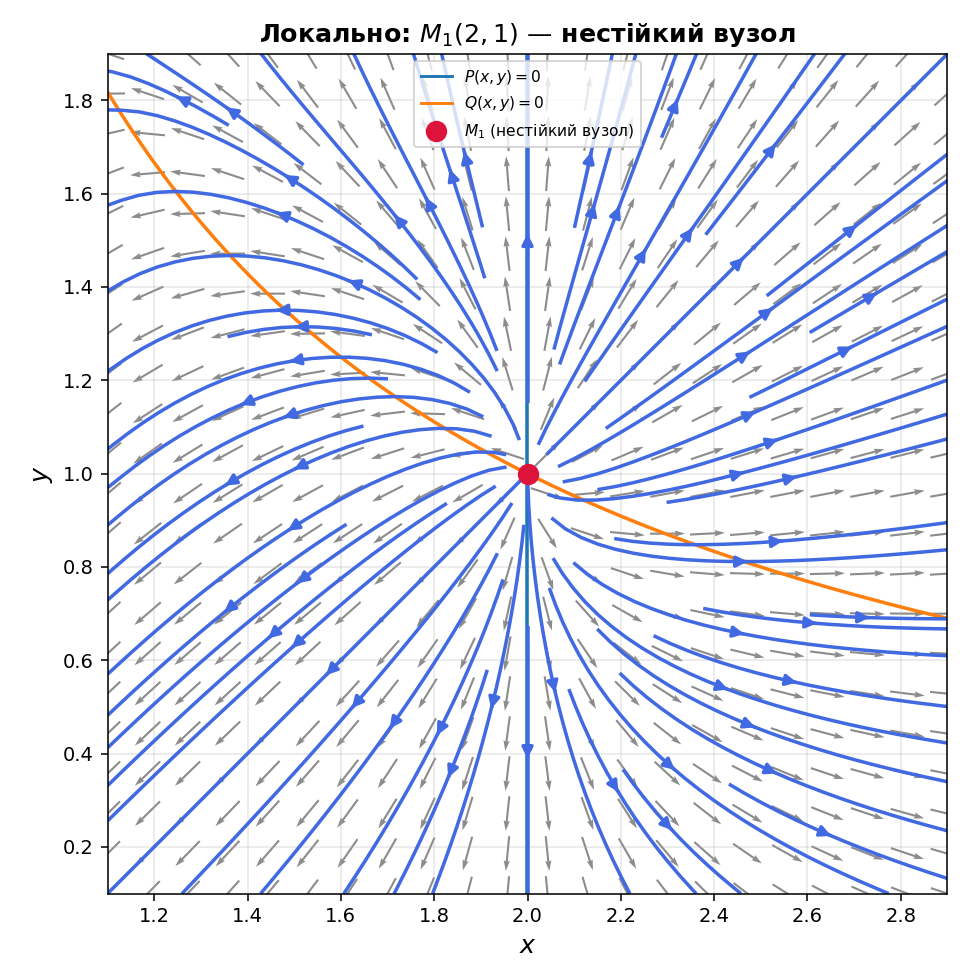
\includegraphics[width=0.48\textwidth]{local_M1.png}
    \caption{Локальний портрет: траєкторії, поле напрямків, криві $\dot{x}=0$ та $\dot{y}=0$; $M_1(2,1)$ --- нестійкий вузол}
\end{figure}


\subsubsection{Лінеаризація в околі $M_2(1,2)$}

\begin{equation*}
J(M_2)=
\begin{pmatrix}
-2 & 1\\
2 & 1
\end{pmatrix}.
\end{equation*}
Характеристичне рівняння:
\begin{equation*}
\begin{vmatrix}
-2-\lambda & 1\\
2 & 1-\lambda
\end{vmatrix}
=\lambda^2+\lambda-4=0,
\end{equation*}
\begin{equation*}
\lambda_{1,2}=\frac{-1\pm\sqrt{17}}{2}\approx 1{,}56,\;\; -2{,}56.
\end{equation*}
Корені дійсні різних знаків --- \textbf{сідло}. Тут $\sigma(1,2)=-1$, $\Delta(1,2)=-4\neq 0$.
Оскільки $\lambda_{1,2}$ дійсні та ненульові, виконана умова теореми Ляпунова про лінійне наближення: локальний портрет вихідної системи в околі $M_2$ топологічно еквівалентний лінеаризованій системі.

Власні напрямки шукаємо у вигляді $s=(\alpha,\beta)^T$ з рівняння $(J-\lambda I)s=0$: з першого рядка $(-2-\lambda)\alpha+\beta=0$, покладемо $\alpha=1$, тоді $\beta=2+\lambda$.
Тобто для $\lambda_+=\dfrac{-1+\sqrt{17}}{2}$ маємо власний вектор $s_+=(1,\;2+\lambda_+)^T$, для $\lambda_-=\dfrac{-1-\sqrt{17}}{2}$ --- $s_-=(1,\;2+\lambda_-)^T$.
У координатах $(x,y)$ сепаратриси лінеаризації мають рівняння прямих через $M_2$ із нахилами $k_\pm = 2+\lambda_\pm = \dfrac{3\pm\sqrt{17}}{2}$.

Напрямок руху на сепаратрисах визначаємо підстановкою пробної точки, яка дещо зміщена від $M_2$ уздовж відповідного власного напрямку, у праві частини системи~\eqref{eq:lab-system37}.

Для $\lambda_+\approx 1{,}56$ маємо $s_+=(1,\;(3+\sqrt{17})/2)\approx(1;\,3{,}56)$. Візьмемо малий зсув $\varepsilon=0{,}1$ уздовж $s_+$:
\begin{equation*}
(x,y)=M_2+\varepsilon\,s_+\approx(1{,}1;\;2{,}356).
\end{equation*}
Підставляючи у~\eqref{eq:lab-system37}:
\begin{align*}
\dot x &= P(1{,}1;\,2{,}356)=(2{\cdot}1{,}1-2{,}356)(1{,}1-2)\approx(-0{,}156)(-0{,}9)\approx 0{,}14>0,\\
\dot y &= Q(1{,}1;\,2{,}356)=1{,}1{\cdot}2{,}356-2\approx 0{,}59>0.
\end{align*}
Вектор $(\dot x,\dot y)$ у цій точці напрямлений «вправо-вгору» --- тобто від $M_2$. Це підтверджує, що $s_+$ --- нестійкий напрямок сідла (траєкторія віддаляється від $M_2$).

Для $\lambda_-\approx -2{,}56$ маємо $s_-=(1,\;(3-\sqrt{17})/2)\approx(1;\,-0{,}56)$. Аналогічно, при $\varepsilon=0{,}1$ пробна точка $M_2+\varepsilon s_-\approx(1{,}1;\,1{,}944)$ дає
\begin{equation*}
\dot x\approx-0{,}23<0,\qquad \dot y\approx 0{,}14>0,
\end{equation*}
тобто вектор $(\dot x,\dot y)$ напрямлений у бік $M_2(1,2)$ --- отже, $s_-$ --- стійкий напрямок (траєкторія наближається до $M_2$).

\begin{figure}[htbp]
    \centering
    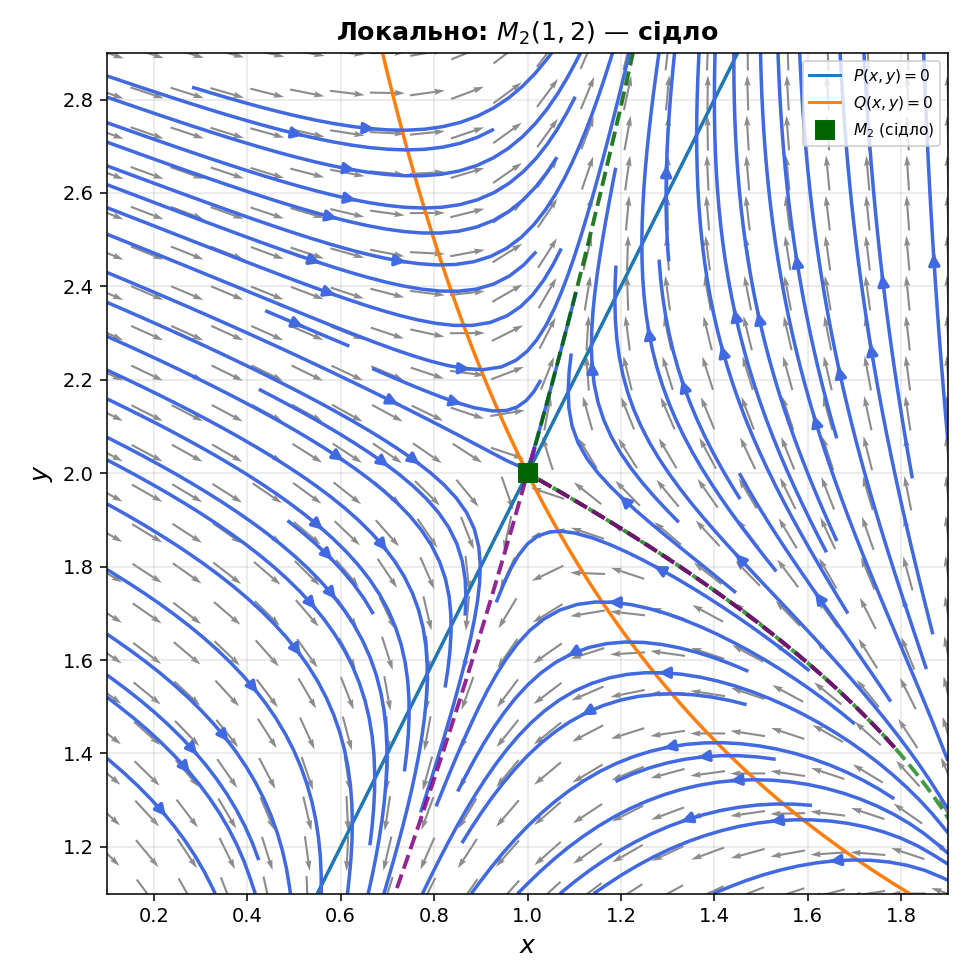
\includegraphics[width=0.48\textwidth]{local_M2.png}
    \caption{Локально біля $M_2(1,2)$ (сідло): траєкторії, поле напрямків, криві $\dot{x}=0$, $\dot{y}=0$, сепаратриси}
\end{figure}


\subsubsection{Лінеаризація в околі $M_3(-1,-2)$}

\begin{equation*}
J(M_3)=
\begin{pmatrix}
-6 & 3\\
-2 & -1
\end{pmatrix}.
\end{equation*}
Характеристичне рівняння:
\begin{equation*}
\lambda^2+7\lambda+12=0,\qquad \lambda_1=-3,\quad \lambda_2=-4.
\end{equation*}
Обидва корені дійсні від'ємні --- \textbf{стійкий вузол}. Маємо $\sigma(-1,-2)=-7$, $\Delta(-1,-2)=12\neq 0$.
Оскільки $\lambda_1,\lambda_2$ дійсні та ненульові, виконана умова теореми Ляпунова про лінійне наближення: локальний портрет вихідної системи в околі $M_3$ топологічно еквівалентний лінеаризованій системі.

Власні вектори шукаємо у вигляді $s=(\alpha,\beta)^T$ з рівняння $(J-\lambda I)s=0$:
\begin{itemize}
    \item для $\lambda=-3$: перший рядок $(J+3I)s=0$ дає $-3\alpha+3\beta=0$, тобто $\alpha=\beta$; беремо $\alpha=1,\beta=1$, звідки $s^{(1)}=(1,1)^T$;
    \item для $\lambda=-4$: перший рядок $(J+4I)s=0$ дає $-2\alpha+3\beta=0$, тобто $\beta=\tfrac{2}{3}\alpha$; беремо $\alpha=3,\beta=2$, звідки $s^{(2)}=(3,2)^T$.
\end{itemize}

\paragraph{Геометрія вузла.}
Загальний розв'язок лінеаризованої системи в координатах $\xi=x+1$, $\eta=y+2$:
\begin{equation*}
\begin{pmatrix}\xi(t)\\ \eta(t)\end{pmatrix}
= C_1\,e^{-3t}\begin{pmatrix}1\\1\end{pmatrix}
+ C_2\,e^{-4t}\begin{pmatrix}3\\2\end{pmatrix}.
\end{equation*}
Менше за модулем власне число --- $\lambda_1=-3$ з \emph{«повільною»} модою та вектором $s^{(1)}=(1,1)^T$ (нахил $1$); більше --- $\lambda_2=-4$ з \emph{«швидкою»} модою і $s^{(2)}=(3,2)^T$ (нахил $2/3$).
При $t\to+\infty$ швидша експонента $e^{-4t}$ згасає першою, тому \textbf{всі траєкторії входять у $M_3$ майже дотично до $s^{(1)}$}; далеко від точки домінує «швидка» мода, тому хвости траєкторій тягнуться уздовж $s^{(2)}$.
Відношення $|\lambda_2|/|\lambda_1|=4/3\approx 1{,}33$ --- невелике, тож вузол \textbf{трохи витягнутий} уздовж $s^{(1)}$ (що і видно на рисунку).

\begin{figure}[htbp]
    \centering
    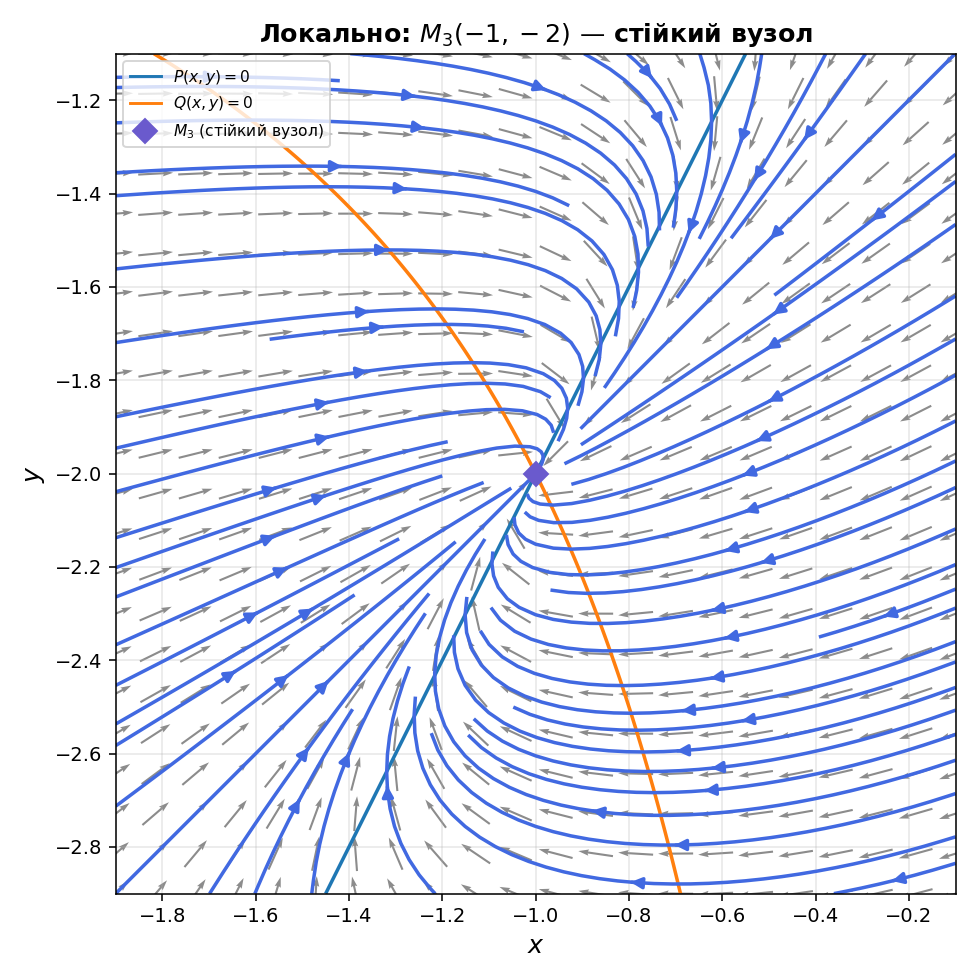
\includegraphics[width=0.48\textwidth]{local_M3.png}
    \caption{Локально біля $M_3(-1,-2)$ (стійкий вузол): траєкторії, поле напрямків та криві $\dot{x}=0$, $\dot{y}=0$}
\end{figure}


\subsubsection{Загальний фазовий портрет}

На рисунку~\ref{fig:lab-global37} зображено фазові траєкторії, вектори $(\dot{x},\dot{y})$ у вузлах сітки та допоміжні криві $P(x,y)=0$, $Q(x,y)=0$ на обраній області.

\begin{figure}[htbp]
    \centering
    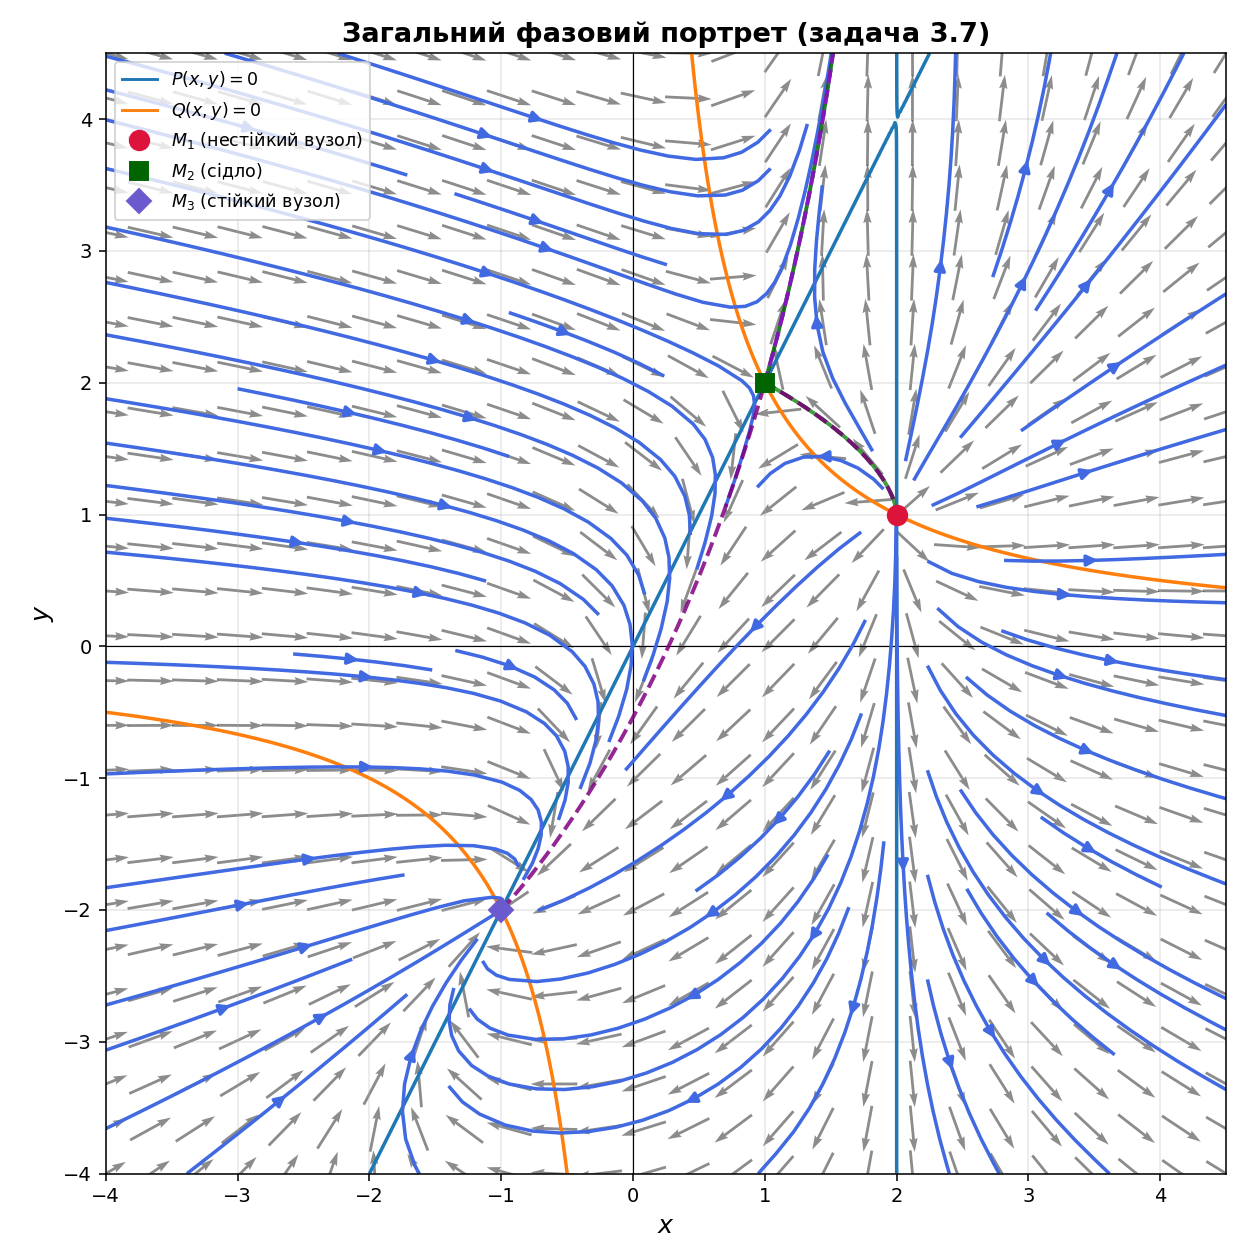
\includegraphics[width=0.48\textwidth]{global_phase_portrait.png}
    \caption{Траєкторії, поле напрямків та криві $\dot{x}=0$, $\dot{y}=0$; система~\eqref{eq:lab-system37}}
    \label{fig:lab-global37}
\end{figure}


\subsubsection{Висновок}

Для системи~\eqref{eq:lab-system37} знайдено три особливі точки $M_1(2,1)$, $M_2(1,2)$, $M_3(-1,-2)$.
Методом лінеаризації встановлено:
\begin{itemize}
    \item $M_1$ --- проста особлива точка типу \textbf{нестійкий вузол} ($\lambda=3,\,2$);
    \item $M_2$ --- \textbf{сідло} ($\lambda_{1,2}=\dfrac{-1\pm\sqrt{17}}{2}$);
    \item $M_3$ --- \textbf{стійкий вузол} ($\lambda=-3,\,-4$).
\end{itemize}
Усі точки прості: $\Delta(x_0,y_0)\neq 0$.
Загальний портрет на рис.~\ref{fig:lab-global37} узгоджується з локальною класифікацією та кривими $P=0$, $Q=0$.

\newpage
\subsection{Завдання 3.6}

\subsubsection{Запис системи}

Розглянемо cтаціонарну систему звичайних диференціальних рівнянь першого порядку на площині:
\begin{equation}\label{eq:lab-system36}
\begin{cases}
\dot{x} = P(x,y) = \ln(2-y^2),\\
\dot{y} = Q(x,y) = e^{x} - e^{y}.
\end{cases}
\end{equation}
\textbf{Область визначення:} $P$ визначена за умови $2-y^2>0$, тобто
\begin{equation*}
D = \{(x,y)\in\mathbb{R}^2 : |y|<\sqrt{2}\} \quad\text{— горизонтальна смуга.}
\end{equation*}
Функція $Q$ визначена й нескінченно диференційовна на всьому $\mathbb{R}^2$; загалом $P,Q\in C^\infty(D)$.

\subsubsection{Знаходження особливих точок}

Особливі точки системи~\eqref{eq:lab-system36} --- розв'язки системи
\begin{equation*}
\ln(2-y^2)=0,\qquad e^{x}-e^{y}=0.
\end{equation*}
З першого рівняння $2-y^2=1$, тобто $y^2=1$, $y=\pm 1$.
З другого, через строге зростання експоненти, $e^x=e^y \Leftrightarrow x=y$.
Звідси дві прості особливі точки:
\begin{equation*}
M_1(1,1),\qquad M_2(-1,-1).
\end{equation*}

\subsubsection{Матриця Якобі та інваріанти лінеаризації}

Частинні похідні:
\begin{align*}
P'_x(x,y) &= 0, &\qquad P'_y(x,y) &= \dfrac{-2y}{2-y^2},\\
Q'_x(x,y) &= e^{x}, &\qquad Q'_y(x,y) &= -e^{y}.
\end{align*}
Матриця Якобі:
\begin{equation}\label{eq:lab-jacobian36}
J(x,y)=
\begin{pmatrix}
0 & -\dfrac{2y}{2-y^2}\\[2mm]
e^{x} & -e^{y}
\end{pmatrix}.
\end{equation}
Слід і визначник:
\begin{equation*}
\sigma(x,y)=-e^{y},\qquad
\Delta(x,y)=\det J(x,y)=0\cdot(-e^{y})-\Bigl(-\dfrac{2y}{2-y^2}\Bigr)\cdot e^{x}
=\dfrac{2y\,e^{x}}{2-y^2}.
\end{equation*}

Як і в задачі~3.7, розкладанням $P,Q$ у ряд Тейлора в околі $(x_0,y_0)$ та перенесенням $x=x_0+\xi$, $y=y_0+\eta$ отримуємо лінеаризовану систему
$\begin{pmatrix}\dot\xi\\ \dot\eta\end{pmatrix}=J(x_0,y_0)\begin{pmatrix}\xi\\ \eta\end{pmatrix}$.

\subsubsection{Лінеаризація в околі $M_1(1,1)$}

Підставимо $(x,y)=(1,1)$ у~\eqref{eq:lab-jacobian36}:
\begin{equation*}
P'_y(1,1)=\dfrac{-2}{2-1}=-2,\quad Q'_x(1,1)=e,\quad Q'_y(1,1)=-e,
\end{equation*}
\begin{equation*}
J(M_1)=
\begin{pmatrix}
0 & -2\\
e & -e
\end{pmatrix}.
\end{equation*}
Маємо $\sigma(1,1)=-e$, $\Delta(1,1)=2e>0$. Характеристичне рівняння:
\begin{equation*}
\lambda^2+e\,\lambda+2e=0,\qquad D=e^2-8e=e(e-8)<0,
\end{equation*}
оскільки $e\approx 2{,}718<8$. Корені --- комплексно-спряжені:
\begin{equation*}
\lambda_{1,2}=\dfrac{-e\pm i\sqrt{\,8e-e^2\,}}{2}
=-\dfrac{e}{2}\pm i\,\dfrac{\sqrt{e(8-e)}}{2}
\approx -1{,}359\pm 1{,}895\,i.
\end{equation*}
Дійсна частина $\operatorname{Re}\lambda_{1,2}=-e/2<0$, тож $M_1$ --- \textbf{стійкий фокус}.
Оскільки $\operatorname{Re}\lambda_{1,2}\neq 0$ і $\lambda_{1,2}\neq 0$, виконана умова теореми Ляпунова про лінійне наближення: локальний портрет вихідної системи в околі $M_1$ топологічно еквівалентний спіралі лінеаризованої системи.

\paragraph{Геометрія спіралі.}
Комплексна пара $\lambda_{1,2}=-\alpha\pm i\omega$ з $\alpha=e/2\approx 1{,}359$ і $\omega=\sqrt{e(8-e)}/2\approx 1{,}895$ задає два характерні масштаби:
\begin{itemize}
    \item \emph{час згасання} $\tau=1/\alpha=2/e\approx 0{,}736$ --- за нього амплітуда радіального відхилення від $M_1$ зменшується в $e\approx 2{,}72$ рази;
    \item \emph{період обертання} $T=2\pi/\omega\approx 3{,}315$ --- час одного повного оберту навколо $M_1$.
\end{itemize}
«Тугість» спіралі визначається відношенням $\alpha/\omega=\sqrt{e/(8-e)}\approx 0{,}717$: за один оберт амплітуда змінюється у $e^{2\pi\alpha/\omega}=\exp\!\bigl(2\pi\sqrt{e/(8-e)}\bigr)\approx e^{4{,}51}\approx 90$ разів. Згасання сильне --- траєкторія практично не встигає зробити повного оберту до того, як наблизиться до $M_1$.

Напрямок обертання визначаємо підстановкою: у точці $M_1+(\varepsilon,0)$ (трохи правіше за $M_1$) маємо $\dot x=P=\ln(2-1^2)=0$, $\dot y=Q=e^{1+\varepsilon}-e\approx\varepsilon\,e>0$, тобто траєкторія в цей момент іде вгору. Отже, обертання --- \textbf{проти годинникової стрілки}.

\begin{figure}[htbp]
    \centering
    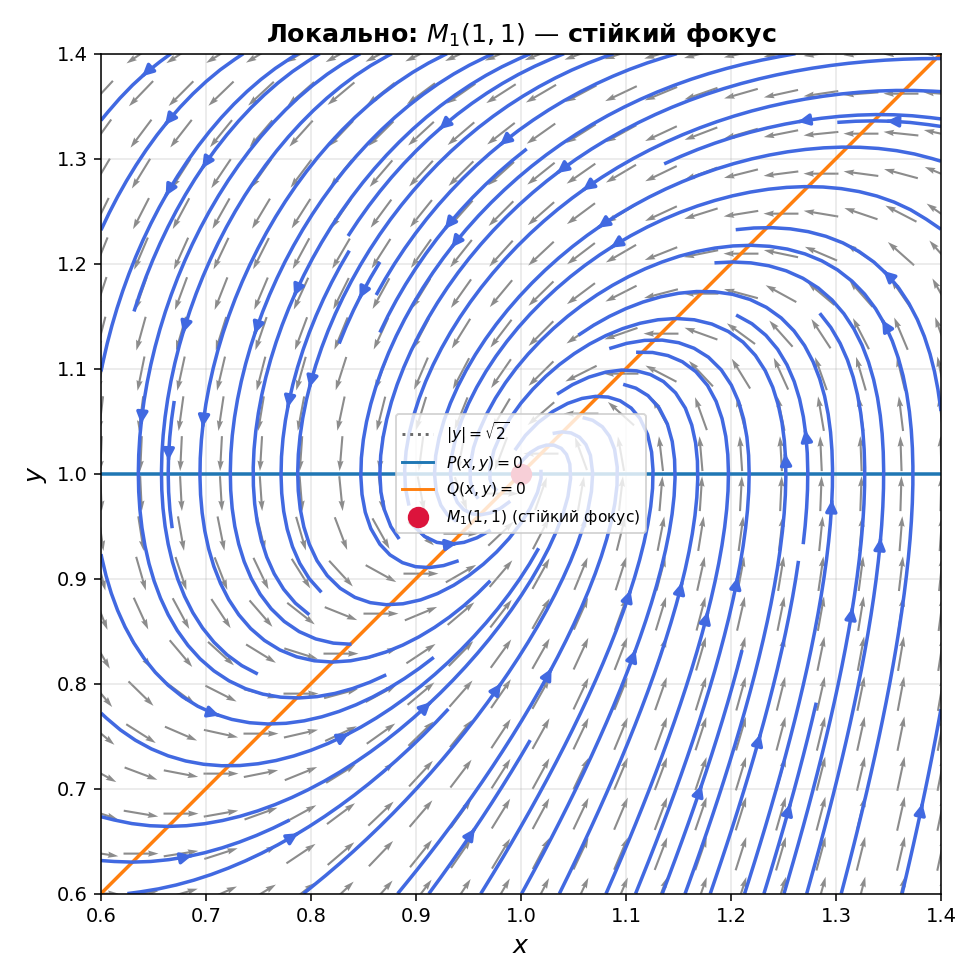
\includegraphics[width=0.48\textwidth]{local_M1_3_6.png}
    \caption{Локально біля $M_1(1,1)$ (стійкий фокус): траєкторії, поле напрямків, криві $\dot{x}=0$, $\dot{y}=0$}
\end{figure}


\subsubsection{Лінеаризація в околі $M_2(-1,-1)$}

Підставимо $(x,y)=(-1,-1)$ у~\eqref{eq:lab-jacobian36}:
\begin{equation*}
P'_y(-1,-1)=\dfrac{-2(-1)}{2-1}=2,\quad Q'_x(-1,-1)=e^{-1},\quad Q'_y(-1,-1)=-e^{-1},
\end{equation*}
\begin{equation*}
J(M_2)=
\begin{pmatrix}
0 & 2\\
\dfrac{1}{e} & -\dfrac{1}{e}
\end{pmatrix}.
\end{equation*}
Маємо $\sigma(-1,-1)=-\dfrac{1}{e}$, $\Delta(-1,-1)=-\dfrac{2}{e}<0$, тому $M_2$ --- \textbf{сідло}. Характеристичне рівняння:
\begin{equation*}
\lambda^2+\dfrac{1}{e}\lambda-\dfrac{2}{e}=0,\qquad
\lambda_{1,2}=\dfrac{-1\pm\sqrt{\,1+8e\,}}{2e}\approx 0{,}693;\;\; -1{,}061.
\end{equation*}
Корені дійсні різних знаків, ненульові --- умова теореми Ляпунова про лінійне наближення виконана; локальний портрет вихідної системи в околі $M_2$ топологічно еквівалентний лінеаризованій системі.

Власні напрямки шукаємо у вигляді $s=(\alpha,\beta)^T$ з рівняння $(J-\lambda I)s=0$. З першого рядка $-\lambda\alpha+2\beta=0$, покладемо $\alpha=1$, тоді $\beta=\lambda/2$, тобто $s=(1,\;\lambda/2)^T$. Нахили сепаратрис лінеаризації:
\begin{equation*}
k_\pm=\dfrac{\lambda_\pm}{2}=\dfrac{-1\pm\sqrt{1+8e}}{4e}.
\end{equation*}
Напрямок руху: вздовж $s_+$ (для $\lambda_+>0$) --- від точки, вздовж $s_-$ (для $\lambda_-<0$) --- до точки.

\begin{figure}[htbp]
    \centering
    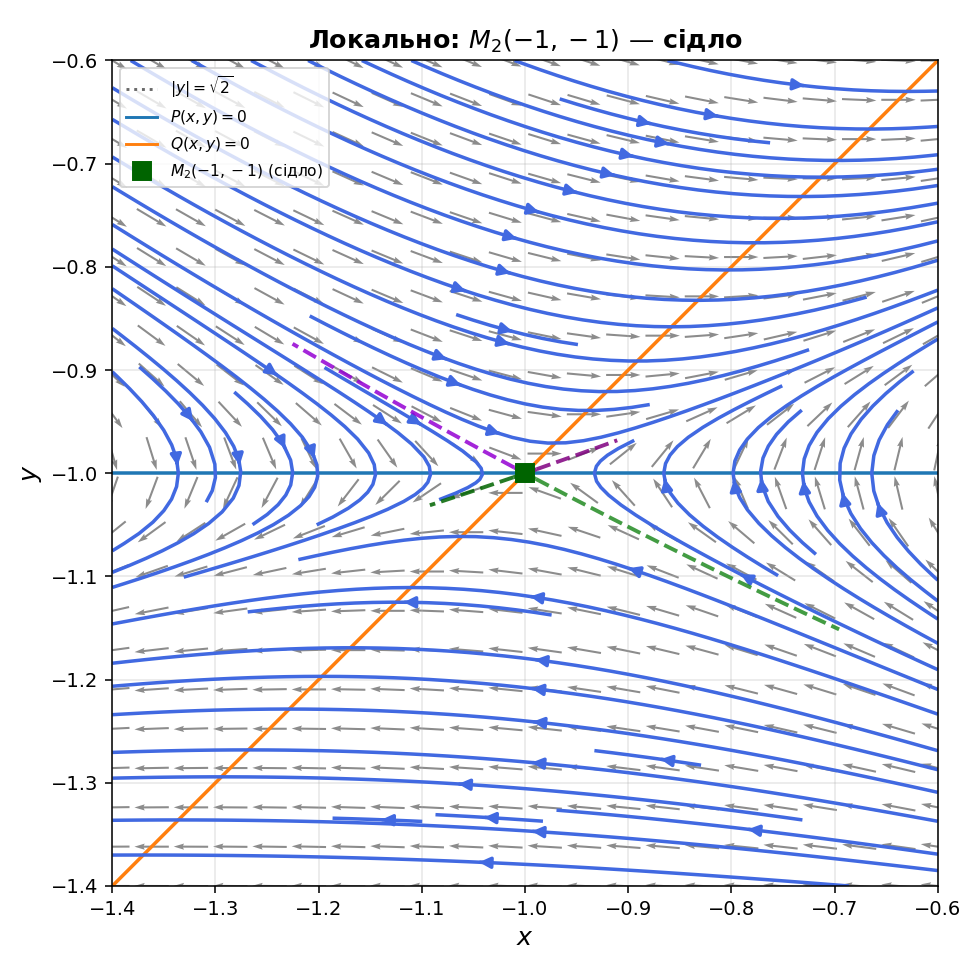
\includegraphics[width=0.48\textwidth]{local_M2_3_6.png}
    \caption{Локально біля $M_2(-1,-1)$ (сідло): траєкторії, поле напрямків, криві $\dot{x}=0$, $\dot{y}=0$ і сепаратриси}
\end{figure}


\subsubsection{Загальний фазовий портрет}

Оскільки функція $P(x,y)=\ln(2-y^2)$ визначена лише в смузі $|y|<\sqrt{2}$, фазовий портрет системи~\eqref{eq:lab-system36} будуємо тільки всередині $D$; прямі $y=\pm\sqrt{2}$ позначено пунктиром як межу області означення.
Криві нульових похідних: $\dot{x}=0$ --- горизонтальні прямі $y=\pm 1$; $\dot{y}=0$ --- бісектриса $y=x$.

\begin{figure}[htbp]
    \centering
    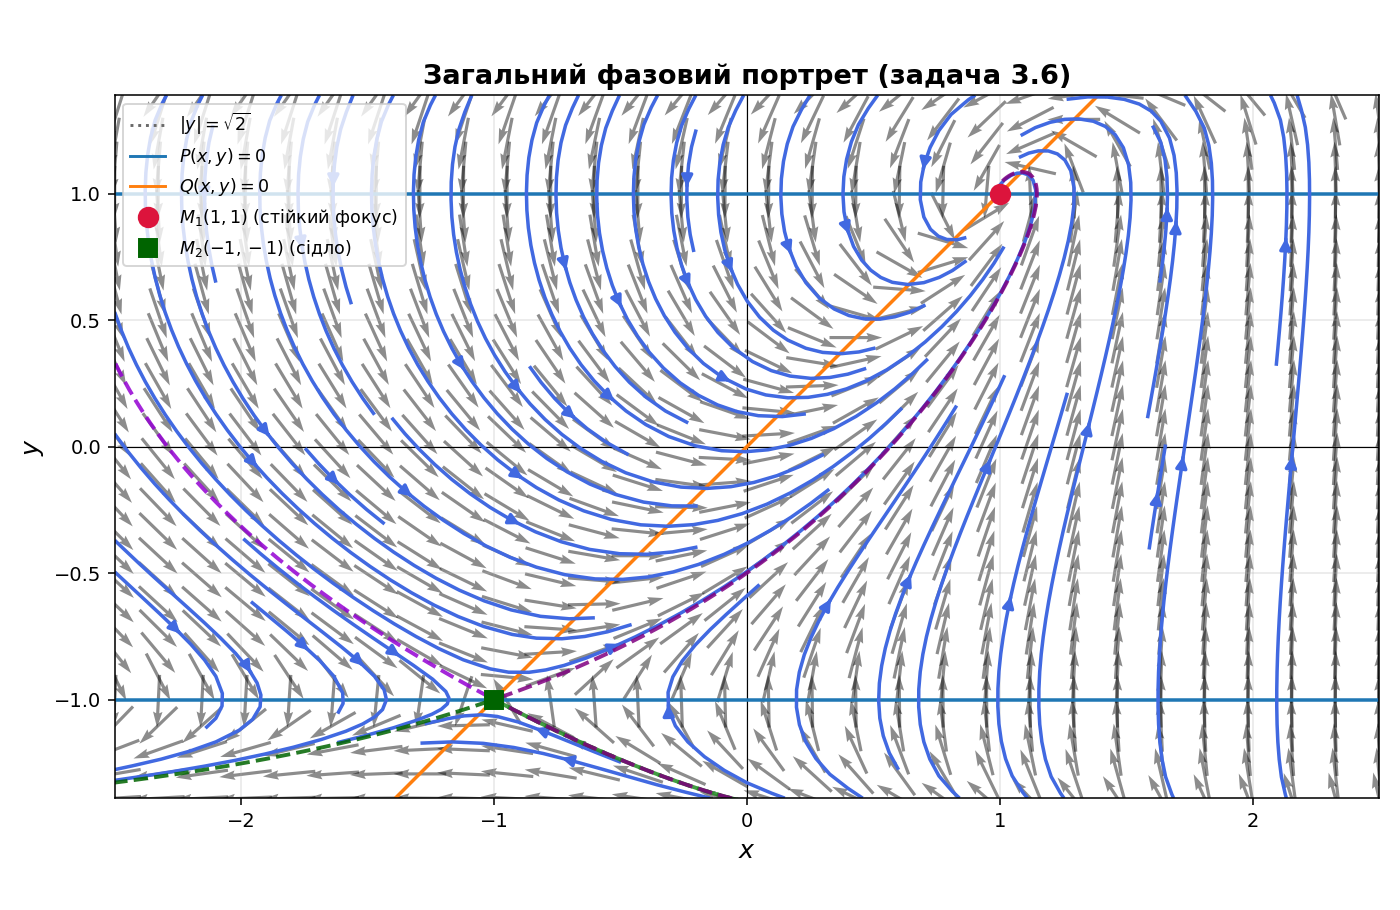
\includegraphics[width=0.48\textwidth]{global_phase_portrait_3_6.png}
    \caption{Загальний фазовий портрет системи~\eqref{eq:lab-system36}: траєкторії, поле напрямків, криві $\dot{x}=0$, $\dot{y}=0$, сепаратриси сідла $M_2$ і межі смуги $|y|=\sqrt{2}$}
    \label{fig:lab-global36}
\end{figure}


\subsubsection{Висновок}

Для системи~\eqref{eq:lab-system36} визначено область означення $|y|<\sqrt{2}$ та знайдено дві особливі точки:
\begin{itemize}
    \item $M_1(1,1)$ --- \textbf{стійкий фокус} ($\lambda_{1,2}=-e/2\pm i\sqrt{e(8-e)}/2$);
    \item $M_2(-1,-1)$ --- \textbf{сідло} ($\lambda_{1,2}=(-1\pm\sqrt{1+8e})/(2e)$).
\end{itemize}
Обидві точки прості: $\Delta(M_1)=2e\neq 0$, $\Delta(M_2)=-2/e\neq 0$.
Загальний фазовий портрет (рис.~\ref{fig:lab-global36}) узгоджується з локальною класифікацією: траєкторії у смузі $|y|<\sqrt{2}$ закручуються навколо стійкого фокуса $M_1$, дві сепаратриси сідла $M_2$ поділяють область на підобласті з різною поведінкою траєкторій.



% =====================================================================
\section{Проблема центра-фокуса}
% =====================================================================

\begin{korotko}
При $\lambda_{1,2}=\pm i\omega$ ($\Delta>0$, $\sigma=0$) лінеаризація дає
\textbf{центр}, але нелінійна система може бути \textbf{фокусом}. Розрізняють
за фокусними величинами $g_k$; для квадратичних систем достатньо $L_1=L_2=L_3=0$
або перевірки гамільтоновості / симетрії.
\end{korotko}

\subsection{Постановка проблеми}

Розглянемо нелінійну автономну систему в околі $(0,0)$:
\begin{equation}\label{eq:center-focus-system}
\begin{cases}
  \dot{x} = ax + by + P(x,y),\\
  \dot{y} = cx + dy + Q(x,y),
\end{cases}
\end{equation}
де $P$, $Q$~--- нелінійні доданки без вільних і лінійних членів.

Матриця Якобі лінеаризованої системи
\begin{equation*}
  J=\begin{pmatrix}a&b\\c&d\end{pmatrix},
\end{equation*}
власні значення $\lambda_1,\lambda_2$ з $\det(J-\lambda E)=0$.

\textbf{Суть проблеми.} Якщо $\lambda_{1,2}=\pm i\omega$ (тобто $\Delta>0$ і
$\sigma=a+d=0$), то для лінеаризованої системи $(0,0)$~--- \textbf{центр}.
Для повної нелінійної системи це \textbf{не гарантує} центр: доданки $P$, $Q$
можуть «закрутити» або «розкрутити» траєкторії, перетворивши точку на
\textbf{стійкий або нестійкий фокус} (складний фокус). Питання «центр чи
фокус?»~--- \textbf{проблема центра-фокуса}; система \emph{негруба}.

\subsection{Полярні координати та фокусні величини}

Перехід $x=r\cos\varphi$, $y=r\sin\varphi$ дає для орбіт рівняння виду
\begin{equation}\label{eq:dr-dphi}
  \frac{dr}{d\varphi}
  = r\,\frac{p_{n+1}(\varphi)+r\,p_{n+2}(\varphi)+r^2 p_{n+3}(\varphi)+\cdots}
         {q_{n+1}(\varphi)+r\,q_{n+2}(\varphi)+r^2 q_{n+3}(\varphi)+\cdots}.
\end{equation}
Шукають сімейство замкнених кривих (аналог функції Ляпунова) у вигляді
формального ряду
\begin{equation}\label{eq:lyapunov-series}
  f(r,\varphi)=r f_0(\varphi)+r^2 f_1(\varphi)+r^3 f_2(\varphi)+\cdots=C.
\end{equation}
Приріст за оберт $0\le\varphi\le2\pi$:
\begin{equation}\label{eq:delta-r}
  \Delta r = g_3 r^4 + g_5 r^6 + g_7 r^8 + \cdots,
\end{equation}
де $g_k$~--- \textbf{ляпуновські} (фокусні) величини.

\textbf{Алгоритм.}
\begin{enumerate}[leftmargin=1.8em]
  \item перша ненульова $g_k<0$ $\Rightarrow$ \textbf{стійкий фокус};
  \item перша ненульова $g_k>0$ $\Rightarrow$ \textbf{нестійкий фокус};
  \item усі $g_k=0$ $\Rightarrow$ \textbf{центр} (замкнені періодичні траєкторії).
\end{enumerate}

\subsection{Достатні умови центра (симетрія)}

Для системи канонічного вигляду
\begin{equation}\label{eq:canonical-center}
\begin{cases}
  \dot{x} = y + P(x,y),\\
  \dot{y} = -x + Q(x,y),
\end{cases}
\end{equation}
якщо фазовий портрет має вісь симетрії через $(0,0)$, то $(0,0)$~---
\textbf{центр}.

\paragraph{Зв'язок із принципом симетрії (§\ref{sec:symmetry}).}
Якщо для
\begin{equation*}
  \frac{dy}{dx}=\frac{-x+Q(x,y)}{y+P(x,y)}
\end{equation*}
виконуються умови симетрії відносно $Ox$ ($y\to-y$) або $Oy$ ($x\to-x$),
фокусні величини обнуляються і точка~--- центр. Заміна $t\to-t$, $y\to-y$
(симетрія відносно $Ox$ і зміна напрямку руху) також гарантує центр.

\subsection{Квадратичні системи}

Система другого степеня в канонічному вигляді:
\begin{equation}\label{eq:quadratic-canonical}
\begin{cases}
  \dot{x} = y + a_{20}x^2 + a_{11}xy + a_{02}y^2,\\
  \dot{y} = -x + b_{20}x^2 + b_{11}xy + b_{02}y^2.
\end{cases}
\end{equation}

\paragraph{Теорема Баутіна.}
$(0,0)$~--- центр у квадратичній системі тоді й лише тоді, коли
\begin{equation}\label{eq:bautin-L}
  L_1=0,\quad L_2=0,\quad L_3=0.
\end{equation}
Якщо~\eqref{eq:bautin-L} виконується, то $L_4,L_5,\ldots$ також нульові.
З особливої точки квадратичної системи при зміні параметрів може виникнути
\textbf{не більше трьох} граничних циклів.

\paragraph{Теорема Каптейна--Дюлака.}
Якщо $(0,0)$~--- центр квадратичної системи, вона \textbf{інтегровна в
квадратурах}: замкнені траєкторії описуються загальним інтегралом або
інтегруючим множником.

\paragraph{Чотири умови центра (Каптейна--Баутіна).}
Центр існує тоді й лише тоді, коли виконується хоча б одна з умов:
\begin{itemize}[leftmargin=1.6em]
  \item \textbf{гамільтоновість:}
        $\operatorname{div}\mathbf{V}\equiv0$,
        $a_{11}+2b_{02}=0$, $b_{11}+2a_{20}=0$;
  \item \textbf{симетрія} фазового портрета (див. вище);
  \item два додаткові алгебраїчні випадки (зведення до рівняння Дарбу,
        спеціальний інтегруючий множник).
\end{itemize}

\subsection{Алгебраїчні умови центра (лекція~5)}

Для систем другого степеня з параметрами $a,b,c,d,\alpha,\beta$ нульовий стан
рівноваги~--- \textbf{центр}, якщо виконується хоча б одна з умов:
\begin{enumerate}[leftmargin=1.8em]
  \item $a+c=0$, \quad $b+d=0$;
  \item $\dfrac{\alpha}{\beta}=\dfrac{b+d}{a+c}=k$,
        $ak^3-(3b+\alpha)k^2+(3c+\beta)k-d=0$;
  \item $\alpha=0$, \quad $\beta=0$;
  \item $a=c=\beta=0$;
  \item $b+d=\alpha=\beta+5a+5c=ac+2a^2+d^2=0$, \quad $(a+c\neq0)$;
  \item $a_1+c_1=\beta_1=\alpha_1+5b_1+5d_1=b_1 d_1+2d_1^2+a_1^2=0$,
        \quad $(b+d\neq0)$,
\end{enumerate}
де $a_1,b_1,c_1,d_1,\alpha_1,\beta_1$~--- коефіцієнти після повороту
\begin{equation*}
  x=x_1\cos\varphi-y_1\sin\varphi,\qquad
  y=x_1\sin\varphi+y_1\cos\varphi,
\end{equation*}
з $\operatorname{tg}\varphi=-\dfrac{a+c}{b+d}$.

\subsection{Практичні критерії}

\textbf{Критерій 1 (гамільтоновість).}
Якщо
\begin{equation}\label{eq:hamilton-div}
  \operatorname{div}\mathbf{V}
  =\frac{\partial P}{\partial x}+\frac{\partial Q}{\partial y}\equiv0,
\end{equation}
то при $\lambda=\pm i\omega$ точка $(0,0)$~--- \textbf{центр}.

\textbf{Критерій 2 (оборотність / симетрія).}
Якщо $\dfrac{dy}{dx}$ інваріантне при $y\to-y$ або $x\to-x$, то $(0,0)$~---
\textbf{центр}.

\subsection{Приклад: перевірка на центр}

\begin{equation}\label{eq:center-example}
\begin{cases}
  \dot{x} = y + x^2 - y^2,\\
  \dot{y} = -x - 2xy.
\end{cases}
\end{equation}

\textbf{Крок 1. Лінеаризація.}
Лінійна частина: $\dot{x}=y$, $\dot{y}=-x$;
$J=\begin{pmatrix}0&1\\-1&0\end{pmatrix}$,
$\lambda_{1,2}=\pm i$~--- для лінеаризованої системи це центр; для повної
системи питання відкрите.

\textbf{Крок 2. Гамільтоновість.}
$P(x,y)=y+x^2-y^2$, $Q(x,y)=-x-2xy$:
\begin{align*}
  \frac{\partial P}{\partial x} &= 2x, &
  \frac{\partial Q}{\partial y} &= -2x,\\
  \operatorname{div}\mathbf{V} &= 2x+(-2x)=0.
\end{align*}

\textbf{Висновок.} За критерієм~\eqref{eq:hamilton-div} точка $(0,0)$~---
\textbf{центр}; обчислювати фокусні величини $g_k$ не потрібно.

% =====================================================================
\section{Критерій Бендіксона}
% =====================================================================

\begin{korotko}
Якщо $\mathrm{div}(P,Q)=P_x+Q_y$ зберігає сталий знак в однозв'язній області $D$,
то в $D$ \textbf{немає} замкнених траєкторій (граничних циклів).
\end{korotko}

Критерій Бендіксона (теорема Бендіксона--Дюлака в простому випадку) дозволяє
довести \textbf{відсутність} замкнених траєкторій у однозв'язній області.

Нехай
\begin{equation}\label{eq:bendixson-system}
\begin{cases}
  \dot{x} = P(x,y),\\
  \dot{y} = Q(x,y).
\end{cases}
\end{equation}

\subsection{Форулювання теореми}

\textbf{Критерій Бендіксона.} Якщо в однозв'язній області $D$ дивергенція поля
\begin{equation}\label{eq:divergence}
  \operatorname{div}\mathbf{V}
  = \frac{\partial P}{\partial x} + \frac{\partial Q}{\partial y}
\end{equation}
зберігає сталий знак (строго $>0$ або строго $<0$, або $=0$ лише в окремих
точках/кривих без зміни знака), то в $D$ \textbf{не існує жодної замкненої
траєкторії}.

\paragraph{Ідея доведення (Грін--Стokes).}
Припустимо, замкнена траєкторія $L$ обмежує область $G\subset D$. За формулою
Гріна:
\begin{equation*}
  \oint_L P\,dy - Q\,dx
  = \iint_G \operatorname{div}\mathbf{V}\,dx\,dy.
\end{equation*}
На $L$ маємо $dx=P\,dt$, $dy=Q\,dt$, тому лівий інтеграл $=\oint(PQ-QP)\,dt=0$.
Якщо $\operatorname{div}\mathbf{V}$ не змінює знак у $G$, подвійний інтеграл
$\neq 0$~--- суперечність.

\subsection{Приклад 1: система загального вигляду}

\begin{equation}\label{eq:bendixson-general}
\begin{cases}
  \dot{x} = y,\\
  \dot{y} = -f(x)y - g(x).
\end{cases}
\end{equation}
Частинні похідні: $P_x=0$, $Q_y=-f(x)$, отже
\begin{equation*}
  \operatorname{div}\mathbf{V} = -f(x).
\end{equation*}
\textbf{Висновок:} якщо в вертикальній смузі $a\le x\le b$ функція $f(x)$
зберігає сталий знак, у цій смузі \textbf{немає} періодичних (замкнених)
траєкторій.

\subsection{Приклад 2: перевірка на всій площині}

\begin{equation}\label{eq:bendixson-explicit}
\begin{cases}
  \dot{x} = x + y^3 + x^3,\\
  \dot{y} = -x + y + y^3.
\end{cases}
\end{equation}

\textbf{Крок 1.} $P(x,y)=x+y^3+x^3$, \quad $Q(x,y)=-x+y+y^3$.

\textbf{Крок 2.} Частинні похідні:
\begin{align*}
  \frac{\partial P}{\partial x} &= 1 + 3x^2, &
  \frac{\partial Q}{\partial y} &= 1 + 3y^2.
\end{align*}

\textbf{Крок 3.} Дивергенція:
\begin{equation*}
  \operatorname{div}\mathbf{V}
  = (1+3x^2) + (1+3y^2) = 2 + 3x^2 + 3y^2.
\end{equation*}

\textbf{Крок 4.} Оскільки $x^2\ge0$, $y^2\ge0$, маємо
$2+3x^2+3y^2\ge 2>0$ для всіх $(x,y)\in\mathbb{R}^2$.

\textbf{Висновок:} за критерієм Бендіксона система~\eqref{eq:bendixson-explicit}
\textbf{не має граничних циклів} на всій фазовій площині.

% =====================================================================
\section{Метод кривих контактів}
% =====================================================================

\begin{korotko}
Топографічна система $F(x,y)=c$; похідна $\dfrac{dF}{dt}=F_x P+F_y Q$ показує,
чи траєкторії входять у криву ($dF/dt<0$), виходять ($>0$), або лежать на ній
($=0$). Класичний вибір: $F=x^2+y^2$.
\end{korotko}

Нехай
\begin{equation}\label{eq:contact-system}
\begin{cases}
  \dot{x} = P(x,y),\\
  \dot{y} = Q(x,y).
\end{cases}
\end{equation}

Розглянемо гладку функцію $F(x,y)$. Сімейство $F(x,y)=c$ ($c=\mathrm{const}$)
утворює \textbf{топографічну систему} замкнених неперетинних кривих.

\subsection{Теорія}

Повна похідна $F$ вздовж траєкторій системи~\eqref{eq:contact-system}:
\begin{equation}\label{eq:dFdt}
  \frac{dF}{dt}
  = \frac{\partial F}{\partial x}\,P(x,y)
  + \frac{\partial F}{\partial y}\,Q(x,y).
\end{equation}
Геометричний зміст на кривій $F(x,y)=c$:
\begin{itemize}[leftmargin=1.6em]
  \item $\dfrac{dF}{dt}<0$~--- траєкторії перетинають криву \textbf{ззовні всередину};
  \item $\dfrac{dF}{dt}>0$~--- \textbf{зсередини назовні};
  \item $\dfrac{dF}{dt}=0$~--- крива складається з траєкторій (наприклад,
        граничний цикл).
\end{itemize}
Метод застосовують для дослідження стійкості, «областей захоплення» та
пошуку циклів (разом із теоремою Пуанкаре--Бендіксона).

\subsection{Приклад 1: коло як крива контакту}

Найпростіша топографічна система~--- кола з центром в $O$:
\begin{equation}\label{eq:contact-circle}
  F(x,y)=x^2+y^2=c \quad (c=R^2>0).
\end{equation}
Тоді
\begin{equation}\label{eq:dFdt-circle}
  \frac{dF}{dt}=2x\,\dot{x}+2y\,\dot{y}=2xP(x,y)+2yQ(x,y).
\end{equation}
Якщо для достатньо великих $R$ маємо $\dfrac{dF}{dt}<0$ на $x^2+y^2=R^2$,
усі траєкторії зовні входять у коло радіуса $R$ і не виходять.

\subsection{Приклад 2: граничний цикл}

\begin{equation}\label{eq:contact-limit}
\begin{cases}
  \dot{x} = y - x(x^2+y^2-1),\\
  \dot{y} = -x - y(x^2+y^2-1).
\end{cases}
\end{equation}

\textbf{Крок 1.} Обираємо $F(x,y)=x^2+y^2=c$ (у правих частинах є $x^2+y^2$).

\textbf{Крок 2.} Обчислюємо $\dfrac{dF}{dt}$:
\begin{align*}
  \frac{dF}{dt}
  &= 2x\bigl[y-x(x^2+y^2-1)\bigr]
   + 2y\bigl[-x-y(x^2+y^2-1)\bigr] \\
  &= 2xy - 2x^2(x^2+y^2-1) - 2xy - 2y^2(x^2+y^2-1) \\
  &= -2(x^2+y^2)(x^2+y^2-1).
\end{align*}

\textbf{Крок 3.} Покладемо $r^2=x^2+y^2$. Тоді $\dfrac{dF}{dt}=-2r^2(r^2-1)$:
\begin{enumerate}[leftmargin=1.6em]
  \item $r<1$: $r^2-1<0$ $\Rightarrow$ $\dfrac{dF}{dt}>0$~--- траєкторії
        \textbf{виходять} зсередини назовні;
  \item $r>1$: $r^2-1>0$ $\Rightarrow$ $\dfrac{dF}{dt}<0$~--- \textbf{входять}
        ззовні всередину;
  \item $r=1$: $\dfrac{dF}{dt}=0$.
\end{enumerate}

\textbf{Висновок:} коло $x^2+y^2=1$~--- \textbf{стійкий граничний цикл};
метод дав існування циклу, і його рівняння.

% =====================================================================
\section{Принцип симетрії}\label{sec:symmetry}
% =====================================================================

\begin{korotko}
Інваріантність $\dfrac{dy}{dx}=\dfrac{Q}{P}$ при $y\to-y$, $x\to-x$ дає
симетрію портрета відносно $Ox$, $Oy$ або $O$. Достатньо будувати портрет у
одній чверті.
\end{korotko}

Нехай
\begin{equation}\label{eq:symmetry-system}
\begin{cases}
  \dot{x} = P(x,y),\\
  \dot{y} = Q(x,y).
\end{cases}
\end{equation}
Рівняння фазових траєкторій:
\begin{equation}\label{eq:phase-ode}
  \frac{dy}{dx} = \frac{Q(x,y)}{P(x,y)}.
\end{equation}
\textbf{Принцип симетрії}~--- перевірка інваріантності~\eqref{eq:phase-ode}
при замінах координат.

\subsection{Симетрія відносно осі $Ox$}

При $y\to-y$, $dy\to-dy$ рівняння не змінюється, якщо
\begin{equation}\label{eq:sym-Ox}
  \frac{Q(x,-y)}{P(x,-y)} = -\frac{Q(x,y)}{P(x,y)}.
\end{equation}
\textbf{Правило:} $P$ \textbf{парна} по $y$ ($P(x,-y)=P(x,y)$), $Q$ \textbf{непарна}
($Q(x,-y)=-Q(x,y)$).

\subsection{Симетрія відносно осі $Oy$}

При $x\to-x$, $dx\to-dx$:
\begin{equation}\label{eq:sym-Oy}
  \frac{Q(-x,y)}{P(-x,y)} = -\frac{Q(x,y)}{P(x,y)}.
\end{equation}
\textbf{Правило:} $P$ \textbf{непарна} по $x$, $Q$ \textbf{парна} по $x$.

\subsection{Симетрія відносно початку $O$}

При $x\to-x$, $y\to-y$ одночасно:
\begin{equation}\label{eq:sym-O}
  \frac{Q(-x,-y)}{P(-x,-y)} = \frac{Q(x,y)}{P(x,y)}.
\end{equation}
Якщо є симетрія відносно обох осей, портрет симетричний і відносно $O$.

\subsection{Приклад: осцилятор Дуффінга без тертя}

\begin{equation}\label{eq:duffing}
\begin{cases}
  \dot{x} = y,\\
  \dot{y} = x - x^3.
\end{cases}
\end{equation}
Тут $P(x,y)=y$, $Q(x,y)=x-x^3$, отже
\begin{equation*}
  \frac{dy}{dx} = \frac{x-x^3}{y}.
\end{equation*}

\textbf{Симетрія відносно $Ox$.}
Заміна $y\to-y$, $dy\to-dy$:
\begin{equation*}
  \frac{-dy}{dx}=\frac{x-x^3}{-y}
  \quad\Longrightarrow\quad
  \frac{dy}{dx}=\frac{x-x^3}{y}.
\end{equation*}
Рівняння збігається~--- портрет \textbf{симетричний відносно $Ox$}.

\textbf{Симетрія відносно $Oy$.}
Заміна $x\to-x$, $dx\to-dx$ (з $(-x)^3=-x^3$):
\begin{equation*}
  \frac{dy}{-dx}=\frac{-x-(-x)^3}{y}=\frac{-x+x^3}{y}
  =-\frac{x-x^3}{y},
\end{equation*}
тобто знову $\dfrac{dy}{dx}=\dfrac{x-x^3}{y}$~--- \textbf{симетрія відносно $Oy$}.

\textbf{Висновок.} Симетрія відносно обох осей $\Rightarrow$ симетрія відносно $O$.
Для повного дослідження достатньо першої чверті ($x\ge0$, $y\ge0$); решту
отримують дзеркальним відображенням~--- це скорочує обсяг роботи приблизно
у 4 рази.

\end{document}
